% \begin{savequote}[8cm]
% Alles Gescheite ist schon gedacht worden.\\
% Man muss nur versuchen, es noch einmal zu denken.

% All intelligent thoughts have already been thought;\\
% what is necessary is only to try to think them again.
%   \qauthor{--- Johann Wolfgang von Goethe \cite{von_goethe_wilhelm_1829}}
% \end{savequote}

\chapter{Theoretical background}
\label{ch:2-litreview}

\minitoc

Some things will need to be said, about \CP violation and such.

\section{The C and P symmetries, and their violation} % (fold)
\label{sec:the_c_and_p_symmetries_and_their_violation}

\begin{itemize}
    \item What does C and P do, fundamentally?
    \item How does that translate to QFTs?
    \item \CP violation historically: kaons, \B physics, now even \D physics!
    \item Three sorts of CP violation, and some early equations on general CP violation (leading on the \KS chapter)
\end{itemize}

% section the_c_and_p_symmetries_and_their_violation (end)

\section{CP violation in the Standard Model} % (fold)
\label{sec:cp_violation_in_the_standard_model}

Then we turn to the SM, where \CP violation is fundamentally included.

\subsection{The CKM matrix and the Unitarity Triangle} % (fold)
\label{sub:the_ckm_matrix}

\begin{itemize}
    \item Define the CKM matrix and count parameters; Wolfenstein parameterisation
    \item How does that give rise to CP violation? Interference is necessary: two sorts. Relate to general discussion earlier
    \item Unitarity constraints and the triangles, pretty pictures..
\end{itemize}

% subsection the_ckm_matrix (end)


\subsection{\texorpdfstring{Measuring the CKM angle $\gamma$ in tree level decays}{Measuring gamma in tree level decays}} % (fold)
\label{sub:_measuring_gamma_in_tree_level_decays}

The amplitude for the decay $\Bm\to\D(\to\KS(\to \pip\pim) \pi^+ \pi^-)\Km$, denoted $\cASm$, can be written as a superposition of the amplitude for a $\Bm\to\Dz\Km$ decay and the suppressed $\Bm\to\Dzb\Km$ decay
\begin{align} \label{eq:A_Bminus}
    \cASm(s_-, s_+)
    &= \AB \AKS \left(\ADS(\smpLong) + \rB \exp[i(\dB - \g)]\ADbS(\smpLong)\right),
\end{align}
where \rB is the ratio of the magnitudes of the $\Bm\to\Dzb\Km$ and $\Bm\to\Dz\Km$ amplitudes, \dB is the strong phase between them, \AB is the amplitude of the $\Bm\to\Dz\Km$ decay.

% subsection _measuring_gamma_in_tree_level_decays (end)

\section{\texorpdfstring{The GGSZ method: measuring $\gamma$ in multi-body \D decays}{The GGSZ method: measuring gamma in multi-body D decays}} % (fold)
\label{sec:the_ggsz_method}

\AKS is the amplitude of the $\KS\to\pip\pim$ decay, \sm and \sp are the squared invariant masses of the $\KS\pim$ and $\KS\pip$ particle combinations, respectively, and the \D decay amplitudes are defined as
\begin{align}\label{eq:ADDb_definition}
\ADorDbSL (\smpLong)= A(\DorDbar^0\to K^0_\text{S(L)} \pi^+\pi^-).
\end{align}
Biases from the effects of $\Dz-\Dzb$ mixing are potentially significant, but can be confined to 0.1$^\circ$ with an appropriate measurement strategy. These effects are described in Ref.~\cite{Dmixing} and are not discussed further in this study. Direct \CP violation in the \D decay is assumed to be negligible, as the effect is expected to be very small for $\D\to\KS\pip\pim$ decays in the SM, and has been analysed in Ref.~\cite{PhysRevD.82.034033}.
Under the further assumption that \KS is a \CP eigenstate, the \D decay amplitudes satisfy 
\begin{align}\label{eq:KS_symmetry}
     \ADbS(\smp)=\ADS(\spm), 
 \end{align} where the short-hand notation $(s_{-+})=(s_-,s_+)$ and $(s_{+-})=(s_+,s_-)$ is employed to simplify equations. The differential $\Bm\to\D(\to\KS \pi^+ \pi^-)\Km$ decay rate to a given point in the \D decay phase space is
\begin{align} \label{eq:Gamma_Bminus}
    \rm {d} \Gamma^-(\smp) &\propto |\cASm|^2 = |\AB|^2|\AKS|^2 \notag \\
    &\qquad\times\left[|\ADS(\smp)|^2 + \rB^2 |\ADS(\spm)|^2 + 2\rB |\ADS(\smp)||\ADS(\spm)|\right .
    \notag \\
    &\quad\qquad \left. \times \left(\cos[-\Delta\delta_D(\smp)]\cos[\dB-\g]-\sin[-\Delta\delta_D(\smp)]\sin[\dB-\g]\right)\right].
\end{align}
Here, $\Delta\delta_\D(\smp) = \delta_D(\smp) - \delta_D(\spm)$, where $\delta_D(\smp)$ denotes the phase of $\ADS(\smp)$. The equivalent expressions to Eq.~\eqref{eq:A_Bminus} and Eq.~\eqref{eq:Gamma_Bminus} for $\Bp\to\D(\to\KS \pi^+ \pi^-)\Kp$ decays are obtained via the substitutions $\g\to-\g$ and $\ADS(\smp)\leftrightarrow\ADbS(\smp)$, where the latter substitution is equivalent to $\ADS(\smp)\leftrightarrow\ADS(\spm)$.


\begin{itemize}
    \item Bring in a high-level discussion of why the phase-space dependence gives a great handle on $\gamma$
    \item Include plots of the phase as a function of phase-space etcetera. Pretty plots can be made using the amplitude model
    \item Do I want to discuss the properties of amplitude models here? It might not actually be a bad idea, because I will need it in a following chapter
    \item Also be explicit about where and why I need the amplitude phase-space symmetry
\end{itemize}

\subsection{A model-independent approach} % (fold)
\label{sub:a_model_independent_approach}


Based on Eq.~\eqref{eq:Gamma_Bminus}, it is possible to measure \g (and the nuisance parameters \rB and \dB) from the phase-space distribution of $\Bpm\to\D(\to\KS \pi^+ \pi^-)\Kpm$ decays, given knowledge of $\delta_D(\smp)$ or $\Delta\delta_D(\smp)$. A series of \g measurements have used amplitude models of the \D decay to describe $\Delta\delta_D(\smp)$ \cite{BABAR2005,BABAR2008,BABAR2010, BELLE2004,BELLE2006,BELLE2010,LHCb-PAPER-2014-017,LHCb-PAPER-2016-007}. More recently, a model-independent approach, which is critical when looking for evidence of beyond-the-SM effects~\cite{BELLEMODIND,LHCb-PAPER-2014-041,LHCb-PAPER-2016-006,LHCb-PAPER-2018-017}, has been favoured. The \D decay phase space is split into $2\times N$ regions, or bins, numbered $i=-N$ to $N$ (omitting zero) that are defined to be symmetric around $\sm=\sp$, with $i>0$ for $s_- >s_+$. The binning scheme used in current experimental measurements of $\Bpm\to\D\Kpm$ decays~\cite{BELLEMODIND,LHCb-PAPER-2014-041,LHCb-PAPER-2018-017} has $N=8$ and is shown in Fig.~\ref{fig:optimal_binning_scheme}. Then, the average of $\cos \Delta\delta_D(\smp)$ over bin $i$ of the \D decay phase space is
\begin{align}\label{eq:ci_si}
    \ci = \frac
    {\int_i \text{d}s^2 |\ADS(\smp)||\ADS(\spm)|\cos[\Delta\delta_D(\smp)]}
    {\sqrt{\int_i \text{d}s^2 |\ADS(\smp)|^2}\sqrt{\int_i \text{d}s^2 |\ADS(\spm)|^2}},
\end{align}
where $\int_i\text{d}s^2$ denotes integration over bin $i$ of the \D decay phase space, and with an analogous definition of \si, the average of $\sin \Delta\delta_D(\smp)$.  Integrating Eq.~\eqref{eq:Gamma_Bminus}, and the corresponding expression for $\Bp\to\D\Kp$ decays, the yields of $\Bpm\to\D(\to\KS \pi^+\pi^-)\Kpm$ in bin $i$ are
\begin{align}
\begin{split}    \label{eq:base_yields}
    N^-_i &= h_B^-\left(\Ki + \rB^2\Kmi + 2\sqrt{\Ki\Kmi}\left(\ci\xm+\si\ym\right)\right), \\
    N^+_i &= h_B^+\left(\Kmi + \rB^2\Ki + 2\sqrt{\Ki\Kmi}\left(\ci\xp-\si\yp\right)\right),
\end{split}
\end{align}
in terms of the integrals 
\begin{align}\label{eq:base_ki}
    K_i &= \frac{1}{N_K}\int_i\text{d}s^2 |\ADS(\smp)|^2, &
    N_K &=\int\text{d}s^2 |\ADS(\smp)|^2,
\end{align}the normalisation constants $h^\pm_B$, and the \CP violation observables ${\xpm = \rB \cos (\dB \pm \g)}$ and $ \ypm = \rB \sin (\dB \pm \g)$.

% \begin{figure}[tb]
%     \centering
%     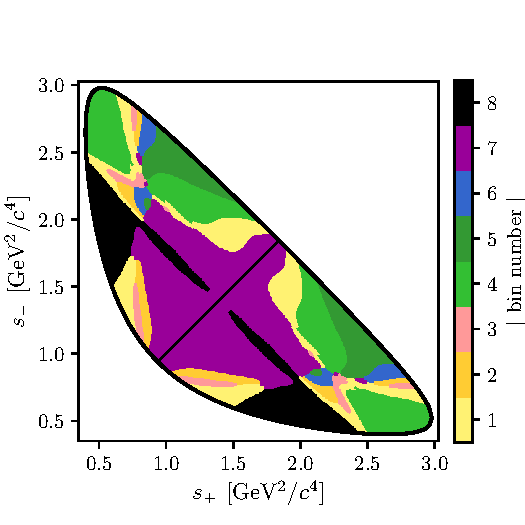
\includegraphics{figures/binning.pdf}
%     \caption{The \emph{optimal binning scheme} of the $\D\to\KS\pip\pim$ phase space~\cite{CLEOCISI}.}
%     \label{fig:optimal_binning_scheme}
% \end{figure}

In model-independent experimental measurements of \g, the signal decay yields in each phase-space bin are expressed via Eq.~\eqref{eq:base_yields} and \xy are determined via a maximum likelihood fit to the data. As Eq.~\eqref{eq:base_yields} leads to 32 observable yields but 36 unknown parameters, it is necessary to use some external information. It is possible to measure \ci and \si using quantum correlated \Dz\Dzb pairs produced at the $\psi(3770)$ resonance \cite{BPMODIND1,BPMODIND2}. Such measurements have been made by the \cleo collaboration~\cite{CLEOCISI}, and these have been employed in a range of \g measurements \cite{BELLEMODIND,LHCb-PAPER-2014-041,LHCb-PAPER-2016-006,LHCb-PAPER-2018-017}. More precise measurements of \ci and \si are expected from the BESIII collaboration, and further measurements could also be made from an analysis of charm mixing \cite{Thomas:2012qf}, or from reconstructed decays of the $\psi(3770)$ meson at LHCb~\cite{Aaij:2019evc}. The \Ki parameters can also be measured in external samples. It is advantageous to determine the \Ki parameters from a sample that has as similar kinematics to the $\Bpm\to\D\Kpm$ sample as possible, in order to automatically include corrections from experimental effects, such as reconstruction efficiency and resolution. A sample of flavour-tagged \D decays is commonly used. Given the current yields of $B$ decays, both the strong phase and \Ki parameters are taken from external input in order to maximise the sensitivity to \xy.     


The interference in $\Bpm\to\D(\to\KS\pi^+ \pi^-)\Kpm$ decays presents itself primarily in different distributions over the \D-decay phase space between signal decays originating from \Bp and \Bm mesons. From an experimental point of view this is highly desirable, as production and detection asymmetries that affect the phase-space-integrated yields can be ignored. In addition to the asymmetry in the distribution over the phase space there is a further \CP asymmetry in the phase-space-integrated yields, expected to be around 1\,\%. This \CP asymmetry is very challenging to measure with useful precision, due to the limited sample sizes currently available and possible biases of a similar magnitude from production and detection asymmetries. Hence, in most studies it is ignored and makes no contribution to the overall determination of \g. 


% subsection a_model_independent_approach (end)

\subsection{Measuring strong-phase inputs at charm factories} % (fold)
\label{sub:measuring_strong_phase_inputs_at_charm_factories}

\begin{itemize}
    \item The thesis should certainly feature a reasonably detailed discussion of how $c_i$ and $s_i$ are actually measured
    \item If I have time, I would like to calculate the impacts of \KS \CP violation and material interaction for these parameters also
\end{itemize}

% subsection measuring_strong_phase_inputs_at_charm_factories (end)

\subsection{Extending the method to multiple decay channels} % (fold)
\label{sub:extending_the_method_to_multiple_decay_channels}

\begin{itemize}
    \item Just a quick definition of the $\xi$ parameters and a reference to Jordi's paper (maybe also Matt's just to show that I know about it)
    \item Important to mention that this is the first time it has been used, what it brings to the table, and that we were the first to carefully show that it works ... 
\end{itemize}

% subsection extending_the_method_to_multiple_decay_channels (end)

% section the_ggsz_method(end)

% section cp_violation_in_the_standard_model (end)